\section{Evaluation of the Proposed Scheme}
\label{sec:counter-evaluation}

We evaluate the counter index on the same machine and in the same run as \cref{sec:evaluation-qpase}
(\cref{tab:machine}). Notebook~07 shows that it works, and notebook~08 measures search time against storage size
for both schemes.

\subsection{Functional results}

Notebook~07 mirrors notebook~03. It stores the same seven files on three servers, at PARAM~I with $N = 3$ and
$t = 2$, so the two notebooks can be read side by side. Each item below is printed by the notebook and checked by
its assertion cells.
\begin{itemize}
  \item \textbf{Rows are small.} A row is a \CiLabelBytes{} label and a \CiEntryBytes{} entry, where the paper's
        index ciphertext $Ct$ is \SizeCt. The Outsource request for the first file is \CiOutsourceRequestBytes, against
        \SizeOutsourceRequest{} for the same file in notebook~03. Most of it is the ML-DSA-44 signature
        (\SizeSigCt).
  \item \textbf{The counter table costs one upload per file.} With four keywords the sealed table fits in one
        1024-byte block and takes \CiSealedBytes. Each Outsource then sends a counter table upload of
        \CiUploadBytes{} to each server.
  \item \textbf{No keyword reaches a server.} The notebook searches every server's stored bytes for each of the
        four keywords and finds none of them.
  \item \textbf{Search returns exactly the matching files.} A search for \texttt{medical} sends one
        \CiSearchRequestBytes{} request with $c_w = 3$ labels to each server. The servers do \CiLookups{} lookups,
        and the label search on all three servers takes \CiRTwoAllServers, against \RTwoAllServers{} for the
        paper's R2 in notebook~03. The user then fetches each file with a \CiFetchRequestBytes{} request and
        recovers items \CiRecoveredItems, byte-equal to the originals and the same items as notebook~03.
  \item \textbf{A stored request misses later uploads.} The notebook keeps the search request, uploads a new
        \texttt{medical} file as item~8, and replays the old request. It finds only items \CiReplayItems. A new
        search asks for one more label and finds items \CiNewSearchItems. In the paper's scheme, by contrast, the
        $\dsk$ kept from one search matches an item uploaded after it.
  \item \textbf{A new device gets the same counters.} A second user object logs in with the same password. At
        L4 the two contacted servers return counter tables with versions \CiNewDeviceVersions. The new device
        rebuilds the first device's table exactly and finds the same four files.
\end{itemize}

\subsection{Search time against storage size}

\paragraph{Setup.} Notebook~08 times one search in both schemes for $N = 3$, 5 and 7 servers and for $10^2$,
$10^3$, $10^4$ and $10^5$ stored files per user, spread evenly over the servers. Each search has $c_w = 3$ matching
files and uses $t = 2$. The three matching files go through the real Outsource and sit on $S_1$, $S_2$ and $S_3$,
one on each. Each run starts with a fresh user object and a fresh Login, so no key or label is cached from an
earlier run. The other files are filler written
straight into server state, because building $10^5$ real files would take hours. For the paper's scheme a filler
item is an AES-256-GCM ciphertext of the real $Ct$'s length under a fresh random key. The server cannot tell it
from another keyword's item, because both fail at the tag check. For the counter index a filler row is a random
label and a random entry of a real entry's length. As in notebook~05, the process is pinned to one CPU, and each
setting runs once as a warm-up and then five times. We report the median. Every timed run checks its result. All
\ScalingChecks{} checked runs returned the right files (\ScalingFailures{} failures), and every counter-index
server did exactly \ScalingLookups{} lookups.

\paragraph{Results.} \Cref{fig:search-scaling} and \cref{tab:search-scaling} give the results. At the slowest
server the counter index took \ScalingIndexMin{} to \ScalingIndexMax{} in every setting. The paper's scheme took
\ScalingPaperMin{} to \ScalingPaperMax. The counter index was therefore \ScalingSpeedupMin{} to
\ScalingSpeedupMax{} times faster at the slowest server, with a median of \ScalingSpeedupMedian{} times. Before
measuring, we expected the paper's search to catch up only at large sizes. There was no crossover. The counter
index searched faster at every size and for every $N$.

\begin{figure}[ht]
\centering
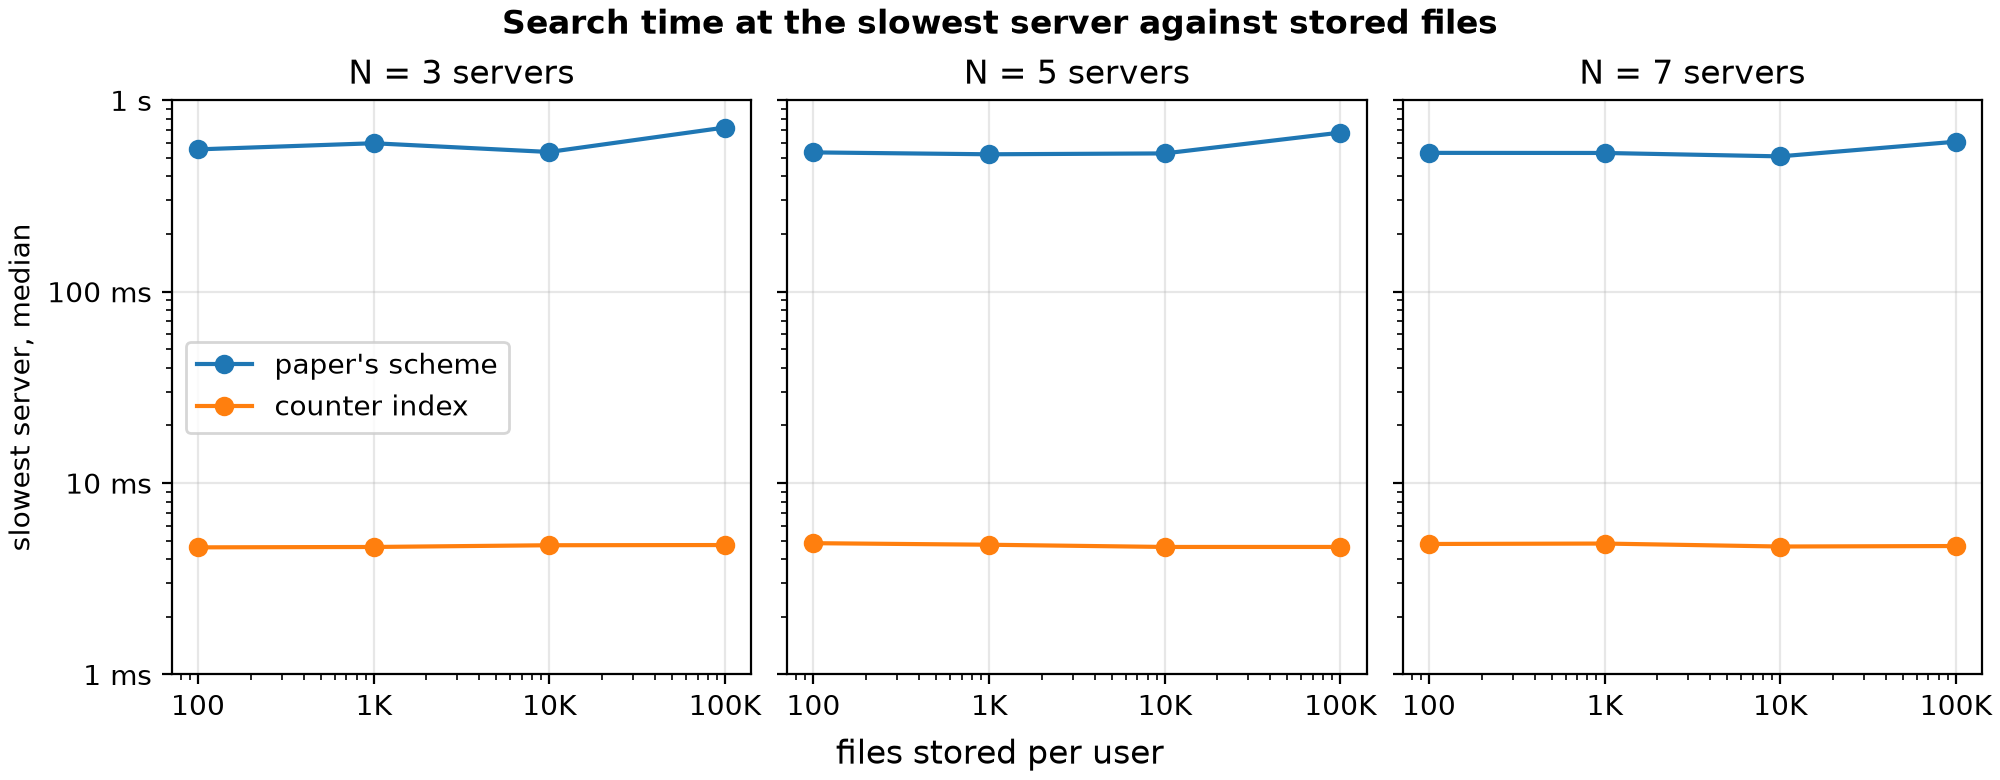
\includegraphics[width=\linewidth]{search_scaling.png}
\caption{Median search time at the slowest server against stored files per user, for $N = 3$, 5 and 7, on log
scales. Each search has three matching files. Drawn by \texttt{notebooks/08\_search\_scaling.ipynb}, cell 7.}
\label{fig:search-scaling}
\end{figure}

\begin{table}[ht]
\centering
\small
\caption{Median search time per setting, over five runs. ``Slowest server'' is the server that took longest in R2,
``all servers'' the sum over the $N$ servers, and ``user'' the user's whole Retrieve. The speed-up is the paper's
slowest server divided by the counter index's. Source: \texttt{notebooks/08\_search\_scaling.ipynb}, cell 7.}
\label{tab:search-scaling}
\resizebox{\linewidth}{!}{% generated by report/tools/make_numbers.py from notebooks/08_search_scaling.ipynb, cell 7
\begin{tabular}{rrrrrrrrr}
\toprule
\textbf{N} & \textbf{files} & \textbf{paper: slowest server} & \textbf{index: slowest server} & \textbf{paper: all servers} & \textbf{index: all servers} & \textbf{paper: user} & \textbf{index: user} & \textbf{speed-up, slowest server} \\
\midrule
3 & 100 & 554 ms & 4.61 ms & 1.66 s & 13.7 ms & 2.21 s & 2.26 s & 120$\times$ \\
3 & 1,000 & 597 ms & 4.64 ms & 1.79 s & 13.9 ms & 2.26 s & 1.93 s & 129$\times$ \\
3 & 10,000 & 537 ms & 4.73 ms & 1.61 s & 14.1 ms & 1.96 s & 2.21 s & 113$\times$ \\
3 & 100,000 & 721 ms & 4.74 ms & 1.93 s & 14.1 ms & 1.98 s & 2.44 s & 152$\times$ \\
5 & 100 & 534 ms & 4.85 ms & 1.61 s & 24.0 ms & 2.14 s & 2.17 s & 110$\times$ \\
5 & 1,000 & 522 ms & 4.76 ms & 1.58 s & 23.6 ms & 2.08 s & 2.13 s & 110$\times$ \\
5 & 10,000 & 528 ms & 4.64 ms & 1.61 s & 22.9 ms & 2.06 s & 2.13 s & 114$\times$ \\
5 & 100,000 & 678 ms & 4.64 ms & 2.08 s & 23.0 ms & 2.33 s & 2.31 s & 146$\times$ \\
7 & 100 & 531 ms & 4.81 ms & 1.61 s & 33.3 ms & 2.13 s & 2.17 s & 111$\times$ \\
7 & 1,000 & 531 ms & 4.83 ms & 1.61 s & 33.2 ms & 2.14 s & 2.18 s & 110$\times$ \\
7 & 10,000 & 510 ms & 4.66 ms & 1.57 s & 32.2 ms & 2.03 s & 2.07 s & 109$\times$ \\
7 & 100,000 & 608 ms & 4.69 ms & 1.95 s & 32.6 ms & 2.34 s & 2.28 s & 130$\times$ \\
\bottomrule
\end{tabular}
}
\end{table}

\paragraph{Where the speed-up comes from.} The speed-up does not come mainly from avoiding a slow scan. A
non-matching item costs the paper's server one failed AES-GCM tag check, which is cheap. Most of the time comes
from the matching items. For each one the paper's server runs one lattice PRF chain to check $v$, and a chain takes
\AxMedian{} (\cref{sec:evaluation-qpase}). The slowest server holds one of the three matches, so it runs one chain. We
infer that this chain makes up most of the paper's slowest-server
time. The counter index's server runs no chain. It verifies one signature and does three lookups. Its time is close
to one ML-DSA-44 verification (\CostVerifyMedian), so we infer that the verification is most of it.

The scan still shows at the largest size. The paper's slowest server rises at $10^5$ files for every $N$. At $N = 3$
it goes from \ScalingPaperThreeTenThousand{} at $10^4$ files to \ScalingPaperThreeHundredThousand{} at $10^5$
files, where each server holds a third of the files. Below $10^5$ files the rise is lost in the cost of the PRF
chain. The counter index stays flat at every size, because a dictionary lookup does not depend on how many rows
the server holds.

\paragraph{All servers together.} Summed over the servers, the paper's scheme took \ScalingPaperSumThree{} at
$N = 3$ and $10^2$ files, about three PRF chains, one for each match. The counter index's sum grows with $N$,
from \ScalingIndexSumThree{} at $N = 3$ to \ScalingIndexSumSeven{} at $N = 7$, because every server verifies the
search request. The speed-up over all servers is therefore smaller at larger $N$. At $10^2$ files it falls from
\ScalingSumSpeedupThree{} times at $N = 3$ to \ScalingSumSpeedupSeven{} times at $N = 7$.

\paragraph{The user's time.} The user's side is about the same in both schemes. Its whole Retrieve took
\ScalingUserPaperMin{} to \ScalingUserPaperMax{} in the paper's scheme and \ScalingUserIndexMin{} to
\ScalingUserIndexMax{} with the counter index. Both run four PRF chains for a search with three matches. In the
paper's scheme the user computes $\dsk$ and then checks $v$ for each returned item. With the counter index it
computes $K_w$ and then one label per match. The counter index moves work off the servers. It does not make a
search faster for the user.
